\documentclass[11pt,t,usepdftitle=false,aspectratio=169]{beamer}
\usepackage{environ}
\usepackage{eqexpl}

% the natbib package allows you to customise your citations 
\usepackage{natbib}


\usetheme[nototalframenumber,foot,logo]{uibk}

%Here I am defining an environment to make my equations look nice
\NewEnviron{myequation}{%
	\begin{displaymath}
		\scalebox{1.2}{$\BODY$}
	\end{displaymath}
}
\eqexplSetDelim{=} 

\title{Example Slides}

\begin{document}
	
	\begin{frame}
		\frametitle{Overview}
		\Large{
			\begin{itemize}
				% with this command, you can determine how far apart items should be for a nicer layout 
				\setlength\itemsep{3mm} 
				\item Motivation
				\item Introduction of the Model 
				\item Solution Concepts 
				\item Real-World Examples 
				\item Evaluation 
		\end{itemize}}
	\end{frame}

\begin{frame}
	\frametitle{Motivation}
	% sometimes centering text can look nice 
	\begin{center}
		\textbf{Reporting security breaches is good...}
	\end{center}
	\begin{itemize}
		\item Users can take action to protect their data from further exploitation
		\item Authorities and other firms can leverage interdependence to prevent further breaches
		\item Mandatory reporting incentivises preventative measures
	\end{itemize}
	\bigskip
	\begin{center}
		% Here \pause is used to display the last part on another slide
		\pause \textbf{... But security breaches are expensive to the companies that are victim to them.\\}
	\end{center}
\end{frame}
	
	\begin{frame}
		\frametitle{Model -- Costs}
		% The minipage is used to split this page into two halves, the image on one side and the formula on the other, each one has its own minipage here 
		\begin{minipage}{0.65\textwidth}
			\textbf{Probability of a Security Breach:} 
			% Here I use displaymath for a formula that appears on its own line 
			\begin{displaymath}
				P_i(x_i, x_{1-i}, t_{1-i})
			\end{displaymath}
			\uncover<5>{\begin{displaymath}
					= 1- (1 - P(x_i)) \cdot (1 - \gamma \cdot P(x_{1-i}) \cdot [1-b\cdot(1-\epsilon)\cdot t_{1-i}]) 
			\end{displaymath}}
			\smallskip % \smallskip, medskip etc. can be used to add some empty space on our page 
			
			% Here I use the myequation environment defined at the beginning of my document in order to have all the = underneath each other 
			\begin{eqexpl}[10mm]\footnotesize
				\setlength\itemsep{0.7mm}
				\uncover<2-5>{\item {\(x_i\)} Security investment of company i}
				\uncover<3-5>{\item {\(x_{1-i}\)} Security investment of other company}
				\uncover<4-5>{\item {\(t_{1-i}\)} Truthful reporting of other company}
				\uncover<5>{\item {\(\gamma \in [0,1]\)} Interdependence between the two companies
					\item {b} Authority's dissemination of knowledge
					\item {$\epsilon$} Error rate of detective controls, fixed at \(\epsilon = 20\%\)}
			\end{eqexpl}
		% I use \uncover here because I want my image to be visible all the time, but the text should appear bit by bit.  
		\end{minipage}
		\hspace{4mm}
		\begin{minipage}{0.30\textwidth}
			\raggedleft
			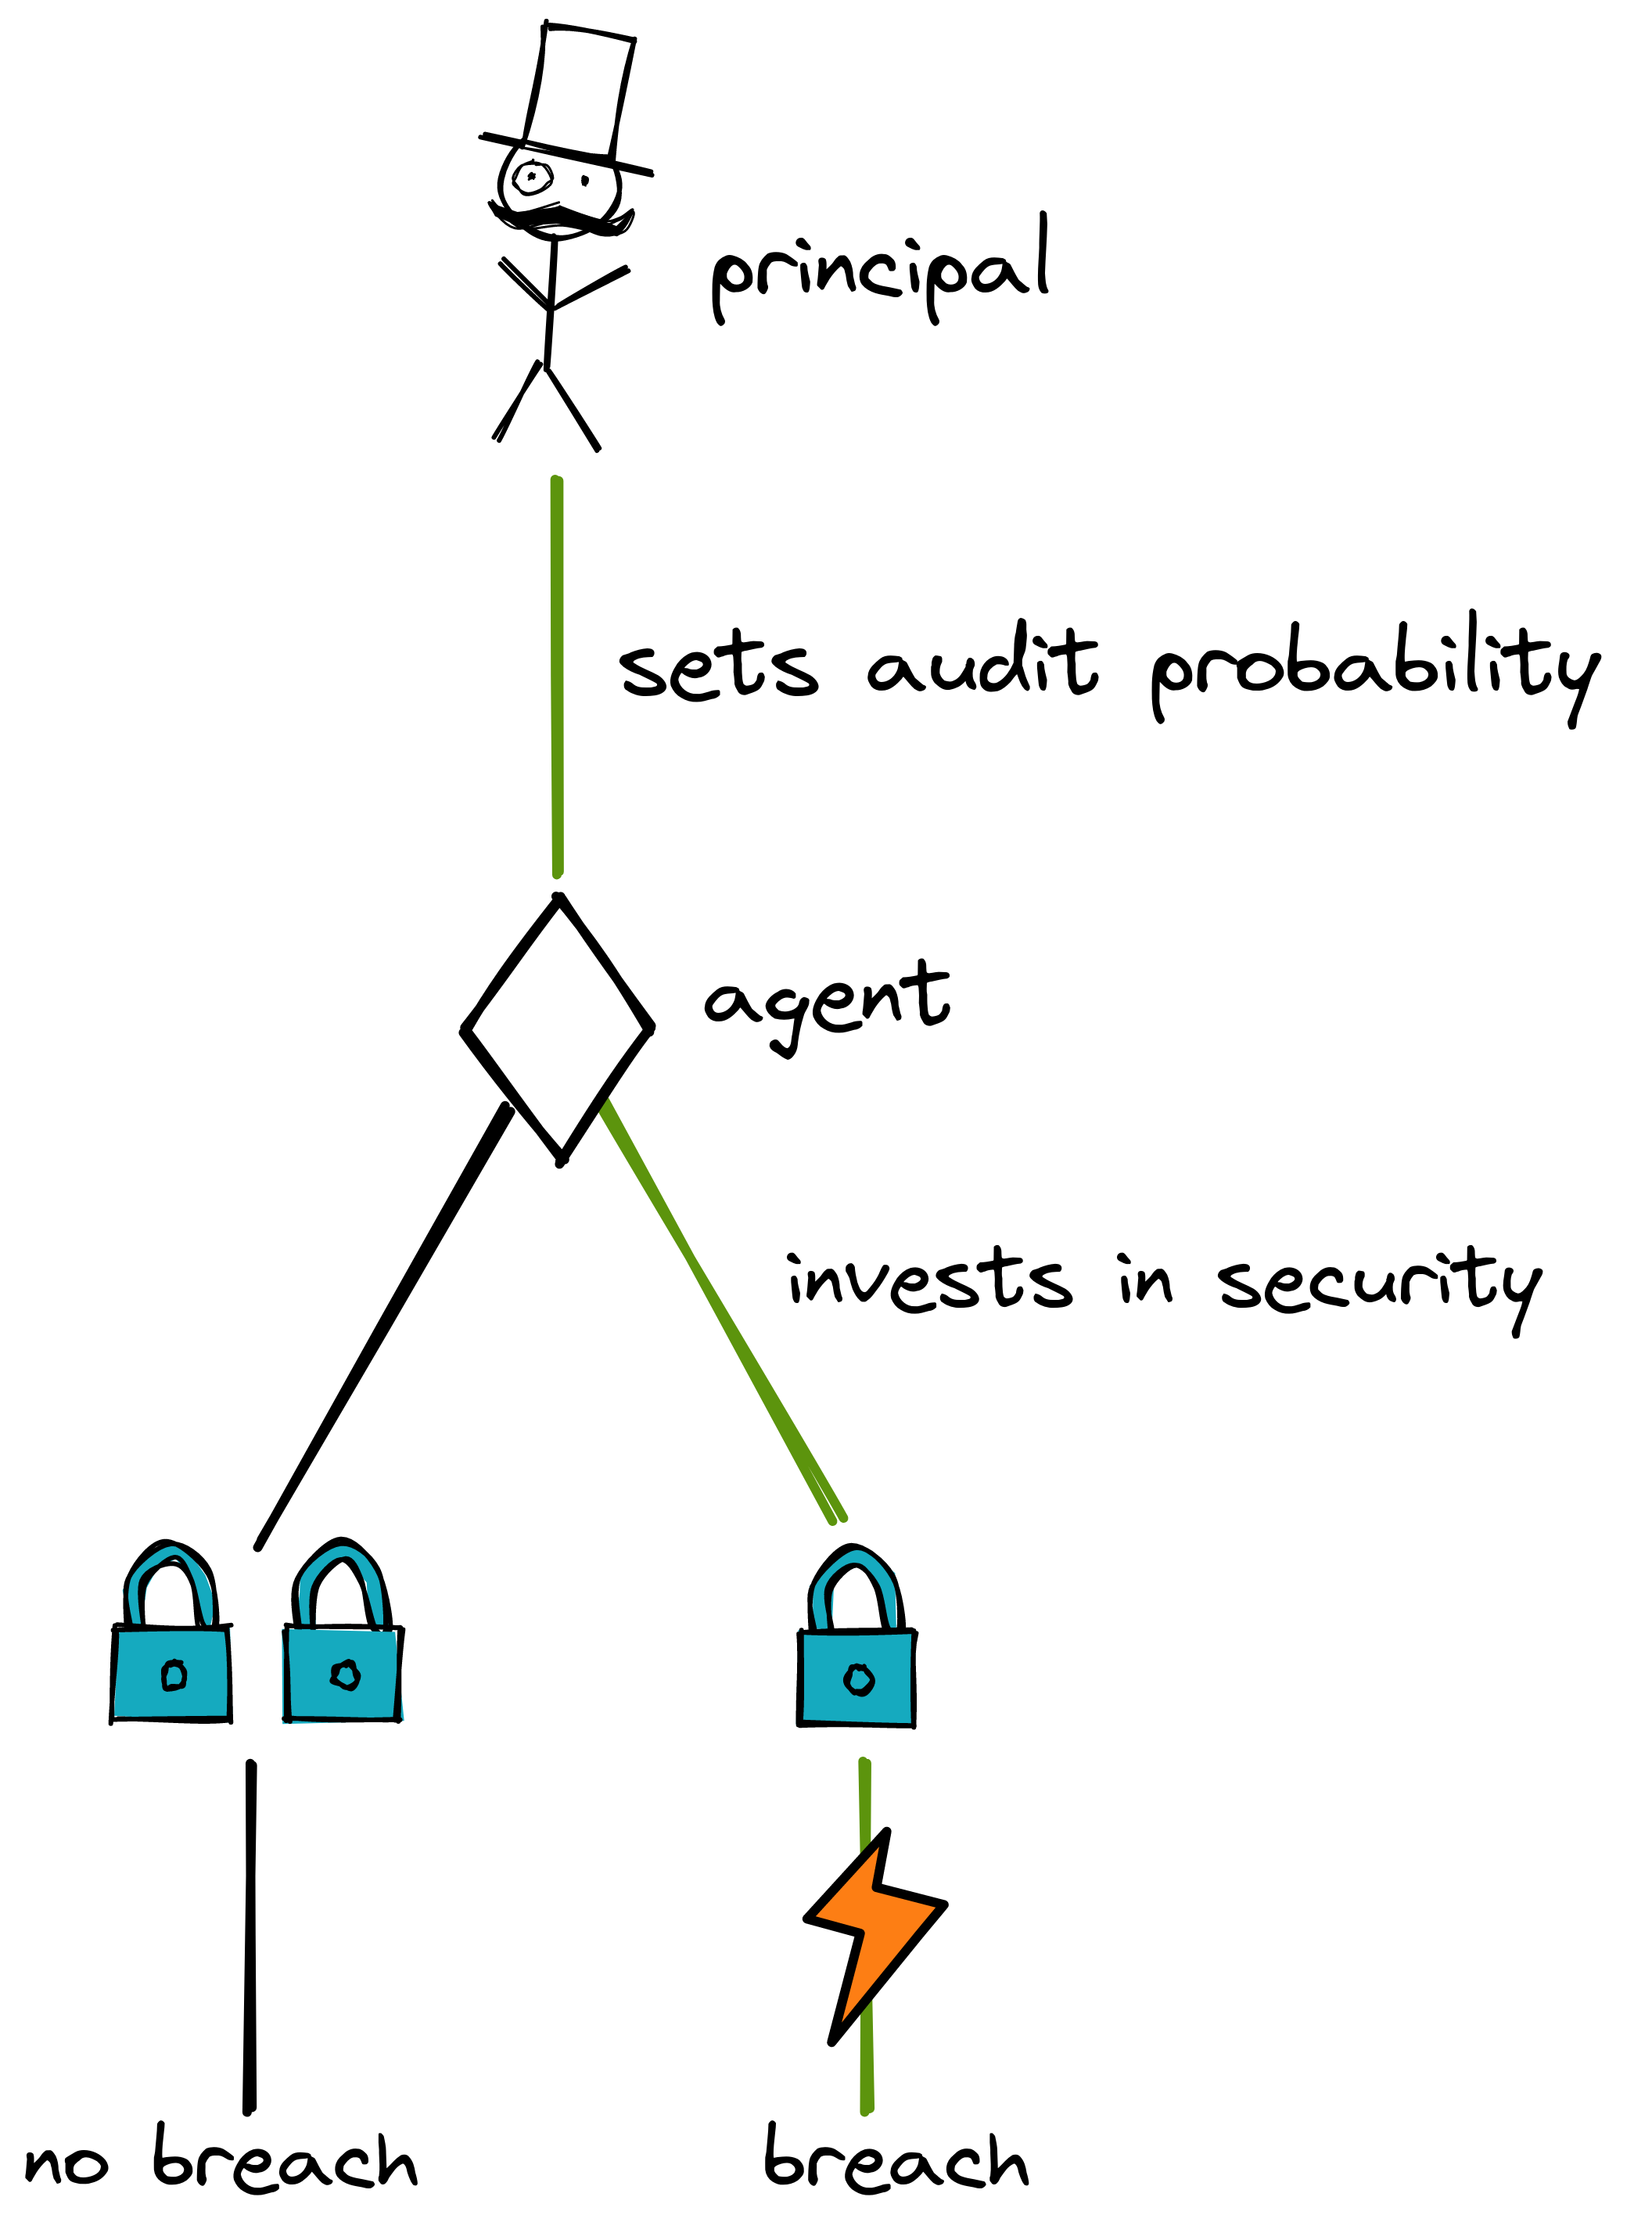
\includegraphics[width=40mm]{model1_3.png}
		\end{minipage}
	\end{frame}


\begin{frame}
	% A nice way to include sources is a bibtex file
	\frametitle{Sources}
	% With the \nocite command, entries are displayed, even if they are not cited in the text itself. This is especially useful in presentations
	\nocite{*}
	\bibliography{bibliography}
	% with this command, you can sort your bibliography, here I went with an unsorted bibliography
	\bibliographystyle{unsrt}
	
	
	
\end{frame}
	
\appendix
	
	\begin{frame}{Appendix: Additional slides}
		The appendix command can be used to create additional slides which will not be listed in the total number of slides \\
		\medskip
		$\rightarrow$ This mainly makes sense if you are displaying the total number of slides you have in your presentation 
	\end{frame}

\end{document}